\documentclass[final]{beamer}
\usepackage{beamerposter}
\usepackage{booktabs}
\usepackage{amssymb}
\usepackage{listings}
\usepackage{courier}
\usepackage{float}
\usepackage{graphicx}
\usepackage{caption}
\usepackage{fontawesome}
\usepackage[scale=2]{ccicons}

% lorem ipsum packages
\usepackage[english]{babel}
\usepackage{blindtext}
\usepackage{lipsum}


% styling commands - template from http://www.latextemplates.com/cat/conference-posters
\usetheme{confposter}
% \setbeamercolor{}{}
\usefonttheme{professionalfonts}
\setbeamerfont{block body}{series=\sffamily}


% layout
% 4-column layout, separation width = 0.008 of paper width
% onecolwid = (1-((4+1)*sepwid))/4 e.g. (1-((4+1)*0.008))/4 = 0.24
% Set twocolwid to be (2*onecolwid)+sepwid = 0.488
\newlength{\sepwid}
\newlength{\onecolwid}
\newlength{\twocolwid}
\setlength{\sepwid}{0.04\paperwidth} % Separation width (white space) between columns
\setlength{\onecolwid}{0.2\paperwidth} % Width of one column
\setlength{\twocolwid}{0.44\paperwidth} % Width of two columns
\setlength{\topmargin}{-0.5in} % Reduce the top margin size


% document metadata
\title{Visualizing Mobile Phone Sensors Data in an R Environment}
\author{Riccardo Miccini}
\institute{Technical University of Denmark - DTU}
\date{\today}


% begin document - single frame, multi-column layout
\begin{document}

\addtobeamertemplate{block end}{}{\vspace*{4ex}} % White space under blocks
\addtobeamertemplate{block alerted end}{}{\vspace*{4ex}} % White space under highlighted (alert) blocks

\begin{frame}[t]
\begin{columns}[t]

	% column 1 - left
	\begin{column}{\onecolwid}
		% objectives
		\begin{alertblock}{Objectives}
			\blindtext
			\blindlist{itemize}[3]
		\end{alertblock}

		% intro
		\begin{block}{\faCommenting \, Introduction}
			\lipsum[66]
			\lipsum[75]
		\end{block}

		% reqs
		\begin{block}{\faListUl \, Requirements}
			\lipsum[75]
			\blindlist{itemize}[5]
		\end{block}
	\end{column}

	% column 2 - center
	\begin{column}{\twocolwid}
		\begin{columns}[t, totalwidth=\twocolwid]
			% column 2.1 - centerleft
			\begin{column}{\onecolwid}\vspace{-.6in}
				% tools
				\begin{block}{\faWrench \, Tools}
					\blindtext
					\blindlist{itemize}[4]
					\lipsum[66]
				\end{block}
			\end{column}

			% column 2.2 - centerright
			\begin{column}{\onecolwid}\vspace{-.6in}
				% implementation
				\begin{block}{\faCode \, Implementation}
					\blindtext
					\lipsum[75]
					\lipsum[66]
				\end{block}
			\end{column}
		\end{columns}

		% main figure section
		\begin{figure}
			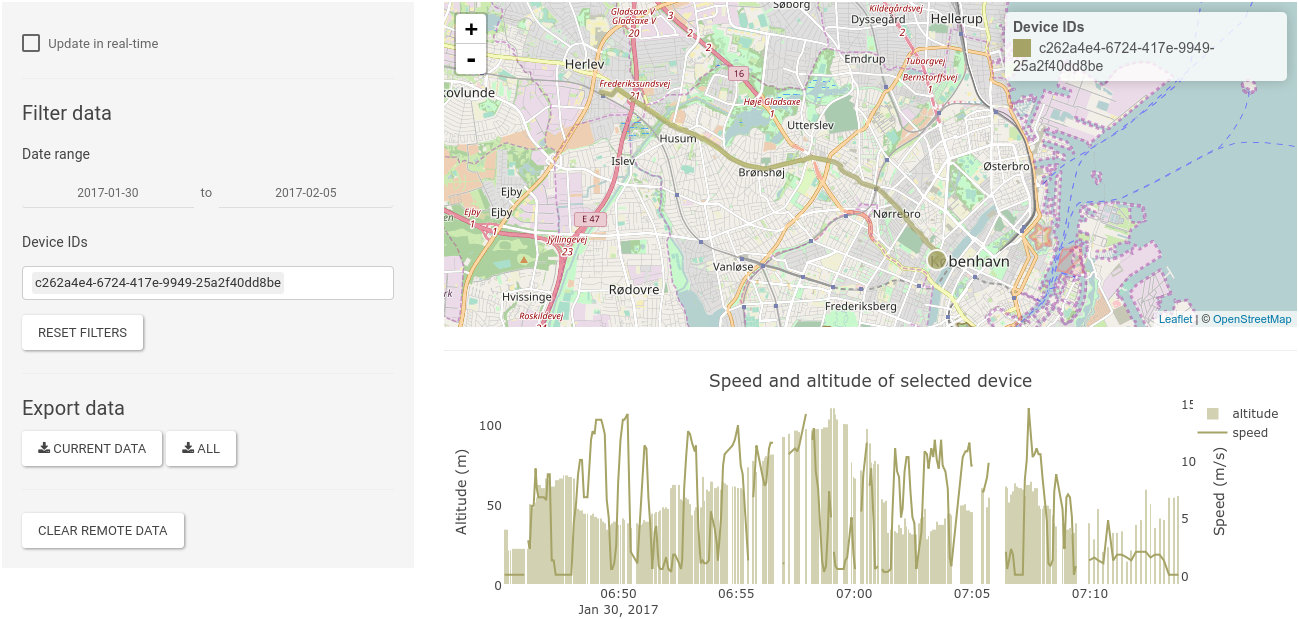
\includegraphics[width=\twocolwid]{ss_ui.png}
			% \caption{Figure caption}
		\end{figure}
	\end{column}

	% column 3 - right
	\begin{column}{\onecolwid}
		% testing
		\begin{block}{\faCheckCircle \, Verification}
			\lipsum[75]
			\lipsum[66]
		\end{block}

		% conclusion
		\begin{block}{\faPieChart \, Results and Conclusion}
			\blindtext
		\end{block}

		% refs
		\begin{block}{\faPaperclip \, References}
			\blindlist{itemize}[5]
			% shiny, leaflet, plotly, dev.android, dev.google
		\end{block}

		% contacts
		\begin{alertblock}{ Conctact Information}
			\faUser \, Riccardo Miccini \\
			\faEnvelope \, s137345@student.dtu.dk \\
			\faGithub \, miccio-dk \\
			\faLinkedin \, rimiccini
		\end{alertblock}

		\begin{center}
			\ccbynd
		\end{center}

	\end{column}



\end{columns}
\end{frame}
\end{document}
